\chapter{Causal inference}\label{chap12}

\section*{Solutions of Exercises}\label{sec12_1}
\begin{enumerate}[leftmargin=*]
\item Show that the Average Treatment Effect (ATE) in the simple linear regression framework
\[
Y_i = \beta_0 + \tau D_i + \mu_i,
\]
assuming non-informative prior distributions, so that the posterior mean of the location parameter coincides with the maximum likelihood estimator, is equal to
\[
\bar{y}_1 - \bar{y}_0.
\]

\textbf{Answer}

Consider the simple linear regression model
\[
Y_i = \beta_0 + \tau D_i + \mu_i, \qquad i = 1,\dots,N,
\]
where $D_i \in \{0,1\}$ is a treatment indicator. In matrix notation:
\[
\mathbf{y} = X \boldsymbol{\beta} + \boldsymbol{\mu}, \qquad
X = \begin{pmatrix}
	1 & D_1 \\
	\vdots & \vdots \\
	1 & D_n
\end{pmatrix}, \quad
\boldsymbol{\beta} = \begin{pmatrix}\beta_0 \\ \tau \end{pmatrix}.
\]

Under the usual Gaussian likelihood and a non-informative prior $\pi(\boldsymbol{\beta},\sigma^2) \propto \sigma^{-2}$, the posterior mean of $\boldsymbol{\beta}$ coincides with the maximum likelihood estimator (MLE), which is the ordinary least squares (OLS) estimator:
\[
\widehat{\boldsymbol{\beta}} = (\mathbf{X}^\top \mathbf{X})^{-1} \mathbf{X}^\top \mathbf{y}.
\]

Compute $\mathbf{X}^\top \mathbf{X}$ and $\mathbf{X}^\top \mathbf{y}$:
\[
\mathbf{X}^\top \mathbf{X} =
\begin{pmatrix}
	N & N_1 \\
	N_1 & N_1
\end{pmatrix}, \qquad
\mathbf{X}^\top \mathbf{y} =
\begin{pmatrix}
	\sum_{i=1}^N y_i \\
	\sum_{i:D_i=1} y_i
\end{pmatrix},
\]
where $N_1 = \sum_i D_i$ and $N_0 = N - N_1$. Let $\bar{y}_1 = \frac{1}{N_1}\sum_{i:D_i=1} y_i$ and $\bar{y}_0 = \frac{1}{N_0}\sum_{i:D_i=0} y_i$.

Compute the inverse:
\[
(\mathbf{X}^\top \mathbf{X})^{-1} =
\frac{1}{N_0 N_1}
\begin{pmatrix}
	N_1 & -N_1 \\
	-N_1 & N
\end{pmatrix}.
\]

Thus:
\[
\widehat{\boldsymbol{\beta}} =
\frac{1}{N_0 N_1}
\begin{pmatrix}
	N_1 & -N_1 \\
	-N_1 & N
\end{pmatrix}
\begin{pmatrix}
	\sum_{i=1}^N y_i \\
	\sum_{i:D_i=1} y_i
\end{pmatrix}
=
\begin{pmatrix}
	\bar{y}_0 \\
	\bar{y}_1 - \bar{y}_0
\end{pmatrix}.
\]

Therefore, the intercept equals the mean outcome for the control group ($\bar{y}_0$), and the slope equals the difference in means between treated and control groups:
\[
\widehat{\tau} = \bar{y}_1 - \bar{y}_0.
\]

Since under a non-informative prior the posterior mean equals the ML estimator, the posterior mean of $\tau$ coincides with the sample difference in means:
\[
\text{ATE} = \mathbb{E}[\tau \mid \mathbf{y}] = \bar{y}_1 - \bar{y}_0.
\]

\item Some readers may question the assumption that potential outcomes are normally distributed. However, it is important to note that the normal distribution is the \textit{maximum entropy} continuous distribution given a specified mean $\mu$ and finite variance $\sigma^2$. In other words, among all distributions with the same mean and variance, the normal distribution represents the one with the greatest level of uncertainty or unpredictability \cite{cover2006elements}.
 
Show that the normal distribution is the \textit{maximum entropy} continuous distribution given a specified mean $\mu$ and finite variance $\sigma^2$ by considering the formal definition of entropy:
\[
H(f) = - \int_{-\infty}^{\infty} f(y) \log f(y) \, dy,
\]
where $f(y)$ is a probability density function.

\textbf{Answer}
  
We want to maximize $H(f)$ subject to the constraints:
\[
\int_{-\infty}^{\infty} f(y)\, dy = 1, \qquad
\int_{-\infty}^{\infty} y f(y)\, dy = \mu, \qquad
\int_{-\infty}^{\infty} (y-\mu)^2 f(y)\, dy = \sigma^2.
\]

Form the Lagrangian:
\[
\mathcal{L}(f) = - \int f(y)\log f(y) \, dy 
+ \lambda_0 \left( \int f(y)\, dy - 1\right)
+ \lambda_1 \left( \int y f(y)\, dy - \mu \right)
+ \lambda_2 \left( \int (y-\mu)^2 f(y)\, dy - \sigma^2 \right).
\]

Taking the functional derivative with respect to $f(y)$:
\[
\frac{\delta \mathcal{L}}{\delta f} = -(\log f(y) + 1) + \lambda_0 + \lambda_1 y + \lambda_2 (y-\mu)^2 = 0.
\]

Thus:
\[
\log f(y) = \lambda_0' + \lambda_1 y + \lambda_2 (y-\mu)^2,
\]
where $\lambda_0'$ absorbs constants. Exponentiating:
\[
f(y) \propto \exp\big( \lambda_1 y + \lambda_2 (y-\mu)^2 \big).
\]

For integrability, $\lambda_2 < 0$. Completing the square:
\[
f(y) \propto \exp\left( -\frac{(y-\mu)^2}{2\sigma^2} \right),
\]
which is the kernel of a normal density. Normalizing:
\[
f(y) = \frac{1}{\sqrt{2\pi\sigma^2}} \exp\left( -\frac{(y-\mu)^2}{2\sigma^2} \right).
\]

Therefore, the maximum entropy distribution for a given mean $\mu$ and variance $\sigma^2$ is
\[
Y \sim N(\mu, \sigma^2).
\]

\item Use the package \textit{dagity} to construct the DAG in Figure~13.5, verify that it is acyclic, and check whether the causal effect of \(D\) on \(Y\) is identifiable by controlling for \(\mathbf{X}\).

\textbf{Answer}

\begin{tcolorbox}[enhanced,width=4.67in,center upper,
	fontupper=\large\bfseries,drop shadow southwest,sharp corners]
	\textit{R code. Simple exercise in \textit{dagity} package: Conditional independence assumption}
	\begin{VF}
		\begin{lstlisting}[language=R]		
library(dagitty)
library(ggdag)

Gd = dagitty('dag{
	X [pos="-1,1"]
	D [exposure, pos="0,0"]
	Y [outcome, pos="1,1"]
	X -> D
	X -> Y
	D -> Y
}')

ggdag(Gd) +  theme_dag()

isAcyclic(Gd)

for( n in names(Gd) ){
	for( m in children(Gd,n) ){
		a <- adjustmentSets(Gd, n, m, effect = c("direct"), type = c("minimal"))
		if( length(a) > 0 ){
			cat("The effect ",n,"->",m,
			" is identifiable by controlling for:\n",sep="")
			print( a, prefix=" * " )
		}
	}
}
\end{lstlisting}
	\end{VF}
\end{tcolorbox} 

\item Use the package \textit{dagitty} to construct the DAG in Figure~13.8, verify that it is acyclic, and check that the causal effect of \(D\) on \(Y\) is identifiable by controlling for \(\mathbf{X}\) but not for \(C\).


\textbf{Answer}

\begin{tcolorbox}[enhanced,width=4.67in,center upper,
	fontupper=\large\bfseries,drop shadow southwest,sharp corners]
	\textit{R code. Simple exercise in \textit{dagity} package: Collider bias}
	\begin{VF}
		\begin{lstlisting}[language=R]		
#### DAG: Collider bias  ####
library(dagitty)
library(ggdag)

Gd = dagitty('dag{
	X [pos="-1,1"]
	D [exposure, pos="0,0"]
	Y [outcome, pos="1,1"]
	C [pos="0,0.5"]
	X -> D
	X -> Y
	X -> C
	D -> Y
	D -> C
}')

ggdag(Gd) +  theme_dag()

isAcyclic(Gd)

adjustmentSets(Gd, exposure = "D", outcome = "Y")

for( n in names(Gd) ){
	for( m in children(Gd,n) ){
		a <- adjustmentSets(Gd, n, m, effect = c("direct"), type = c("minimal"))
		if( length(a) > 0 ){
			cat("The effect ",n,"->",m,
			" is identifiable by controlling for:\n",sep="")
			print( a, prefix=" * " )
		}
	}
}
\end{lstlisting}
	\end{VF}
\end{tcolorbox}

\item Use the package \textit{dagitty} to construct the DAG in Figure~13.11, taking into account that $\mathbf{U}$ is unobserved (latent). Verify that it is acyclic, check that $Z$ is a valid instrument, and determine whether the causal effect of \(D\) on \(Y\) is identifiable.

\textbf{Answer}

\begin{tcolorbox}[enhanced,width=4.67in,center upper,
	fontupper=\large\bfseries,drop shadow southwest,sharp corners]
	\textit{R code. Simple exercise in \textit{dagity} package: Instrumental variable}
	\begin{VF}
		\begin{lstlisting}[language=R]		
#### DAG: Instruments  ####
library(dagitty)
library(ggdag)

Gd = dagitty('dag{
	U [latent, pos="-1,1"]
	D [exposure, pos="0,0"]
	Y [outcome, pos="1,1"]
	Z [pos="0,0.5"]
	U -> D
	U -> Y
	D -> Y
	Z -> D
}')

ggdag(Gd) +  theme_dag()

isAcyclic(Gd)

instrumentalVariables(Gd)

adjustmentSets(Gd, exposure = "D", outcome = "Y")
\end{lstlisting}
	\end{VF}
\end{tcolorbox}


\item \textbf{401(k) participation on net financial assets continues I}  

Apply the framework from this example to compute the intention-to-treat effect, the local average treatment effect, and the effect of eligibility on participation.

\textbf{Answer}

Taking into account that
\begin{align*}
	\tau_{LATE} &= \mathbb{E}[Y_i(1)-Y_i(0)\mid D(1)=1, D(0)=0] \\
	&= \frac{\mathbb{E}[Y_i \mid Z_i=1] - \mathbb{E}[Y_i \mid Z_i=0]}{\mathbb{E}[D_i \mid Z_i=1] - \mathbb{E}[D_i \mid Z_i=0]},
\end{align*}
we can recover the ITT effect by multiplying the LATE by the effect of eligibility on participation. The following code illustrates this procedure and plots the ITT. The posterior distribution of the ITT is shown in Figure \ref{fig12_1}, which closely resembles the posterior distribution of the effect of eligibility reported in the main text.

\begin{tcolorbox}[enhanced,width=4.67in,center upper,
	fontupper=\large\bfseries,drop shadow southwest,sharp corners]\label{code1_chap12}
	\textit{R code. Treatment effect: 401(k) participation on net financial assets}
	\begin{VF}
		\begin{lstlisting}[language=R]		
rm(list = ls()); set.seed(10101)
library(coda); library(ggplot2)
mydata <- read.csv("https://raw.githubusercontent.com/BEsmarter-consultancy/BSTApp/refs/heads/master/DataApp/401k.csv", sep = ",", header = TRUE, quote = "")
# Attach variables
attach(mydata)
y <- net_tfa/1000  # Outcome: net financial assets
x <- as.vector(p401) # Endogenous regressor: participation
w <- as.matrix(cbind(1, age, inc, fsize, educ, marr, twoearn, db, pira, hown))  # Exogenous regressors with intercept
z <- as.matrix(e401)  # Instrument: eligibility (NO intercept here)
X <- cbind(x, w); Z <- cbind(z, w)
# Dimensions
k <- ncol(X); kz <- ncol(Z)  
# Priors
b0 <- rep(0, k); B0i <- diag(1e-5, k)
g0 <- rep(0, kz); G0i <- diag(1e-5, kz)
nu <- 3; Psi0 <- nu * 1000 * diag(2); Psi0i <- solve(Psi0)
# MCMC parameters
mcmc <- 5000; burnin <- 1000
tot <- mcmc + burnin; thin <- 1
# Auxiliary elements
XtX <- t(X)%*%X; ZtZ <- t(Z)%*%Z; nun <- nu + length(y)
# Gibbs sampling
PostBeta <- function(Sigma, Gamma){
	w1 <- Sigma[1,1] - Sigma[1,2]^2/Sigma[2,2]
	Bn <- solve(w1^(-1)*XtX + B0i)
	yaux <- y - (Sigma[1,2]/Sigma[2,2])*(x - Z%*%Gamma)
	bn <- Bn%*%(B0i%*%b0 + w1^(-1)*t(X)%*%yaux)
	Beta <- MASS::mvrnorm(1, bn, Bn)
	return(Beta)
}
PostGamma <- function(Sigma, Beta){
	w2 <- Sigma[2,2] - Sigma[1,2]^2/Sigma[1,1]
	Gn <- solve(w2^(-1)*ZtZ + G0i)
	xaux <- x - (Sigma[1,2]/Sigma[1,1])*(y - X%*%Beta)
	gn <- Gn%*%(G0i%*%g0 + w2^(-1)*t(Z)%*%xaux)
	Gamma <- MASS::mvrnorm(1, gn, Gn)
	return(Gamma)
}
PostSigma <- function(Beta, Gamma){
	Uy <- y - X%*%Beta; Ux <- x - Z%*%Gamma
	U <- cbind(Uy, Ux)
	Psin <- solve(Psi0i + t(U)%*%U)
	Sigmai <- rWishart::rWishart(1, df = nun, Sigma = Psin)
	Sigma <- solve(Sigmai[,,1]) 
	return(Sigma)
}
\end{lstlisting}
	\end{VF}
\end{tcolorbox} 

\begin{tcolorbox}[enhanced,width=4.67in,center upper,
	fontupper=\large\bfseries,drop shadow southwest,sharp corners]\label{code1a_chap12}
	\textit{R code. Treatment effect: 401(k) participation on net financial assets}
	\begin{VF}
		\begin{lstlisting}[language=R]		
ITT <- Bs[,1]*Gs[,1]
summary(coda::mcmc(ITT))
# Convert to data frame for ggplot
df_ITT <- data.frame(ITT = as.vector(ITT))

# Plot posterior distribution of treatment effect
ggplot(df_ITT, aes(x = ITT)) + geom_density(fill = "steelblue", alpha = 0.6) +
geom_vline(xintercept = mean(ITT), color = "red", linetype = "dashed", linewidth = 1) + labs(title = "Posterior Distribution of 401(k) ITT", x = expression(beta["ITT"]), y = "Density") + theme_minimal(base_size = 14)
\end{lstlisting}
	\end{VF}
\end{tcolorbox} 

\begin{figure}[h!]
	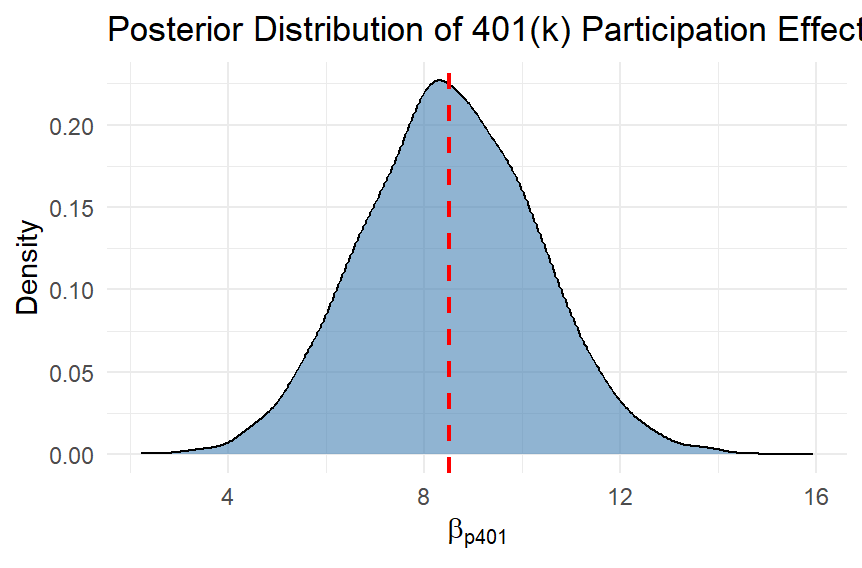
\includegraphics[width=340pt, height=200pt]{Chapters/chapter12/figures/FigP401k.png}
	\caption[List of figure caption goes here]{Posterior distribution: Intention-to-treat effect 401k participation on net financial assets.}\label{fig12_1}
\end{figure}

\item \textbf{401(k) participation on net financial assets continues II} 

Perform inference in this example assuming that the stochastic errors follow a Dirichlet process, using the function \textit{rivDP} from the \textit{bayesm} package to analyze 401(k) participation and its effect on net financial assets under the same specification as in the main text, and plot the LATE.

\textbf{Answer}

The following code implements the exercise, and Figure \ref{fig12_2} display the posterior distribution of the LATE. The results are very similar to the ones in the main text assuming a normal distribution; however, the degree of dispersion of higher using a Dirichlet process for the stochastic errors.  

\begin{tcolorbox}[enhanced,width=4.67in,center upper,
	fontupper=\large\bfseries,drop shadow southwest,sharp corners]
	\textit{R code. Treatment effect: 401(k) participation on net financial assets using Dirichlet process}
	\begin{VF}
		\begin{lstlisting}[language=R]		
rm(list = ls()); set.seed(10101)
library(ggplot2); library(bayesm)
# Load data
mydata <- read.csv("https://raw.githubusercontent.com/BEsmarter-consultancy/BSTApp/refs/heads/master/DataApp/401k.csv",
sep = ",", header = TRUE, quote = "")
# Attach variables
attach(mydata)
y <- net_tfa/1000     # Outcome: net financial assets
x <- as.vector(p401)  # Endogenous regressor: participation
w <- as.matrix(cbind(age, inc, fsize, educ, marr, twoearn, db, pira, hown))  # Exogenous regressors with intercept
z <- as.matrix(e401)  # Instrument: eligibility (NO intercept here)

# specify data input and mcmc parameters
Data = list(); 
Data$z <- z
Data$x <- x
Data$y <- y
Data$w <- w

Mcmc = list()
Mcmc$maxuniq <- 100
Mcmc$R <- 5000
keep <- seq((1000+1), Mcmc$R)

out <- rivDP(Data=Data, Mcmc=Mcmc)

# Plot posterior distribution of treatment effect
df_ITT <- data.frame(ITT = out[["betadraw"]][kepp])
ggplot(df_ITT, aes(x = ITT)) + geom_density(fill = "steelblue", alpha = 0.6) + geom_vline(xintercept = mean(ITT), color = "red", linetype = "dashed", linewidth = 1) + labs(title = "Posterior Distribution of 401(k) ITT: Dirichlet process", x = expression(beta["ITT"]), y = "Density") + theme_minimal(base_size = 14)
\end{lstlisting}
	\end{VF}
\end{tcolorbox} 

\begin{figure}[h!]
	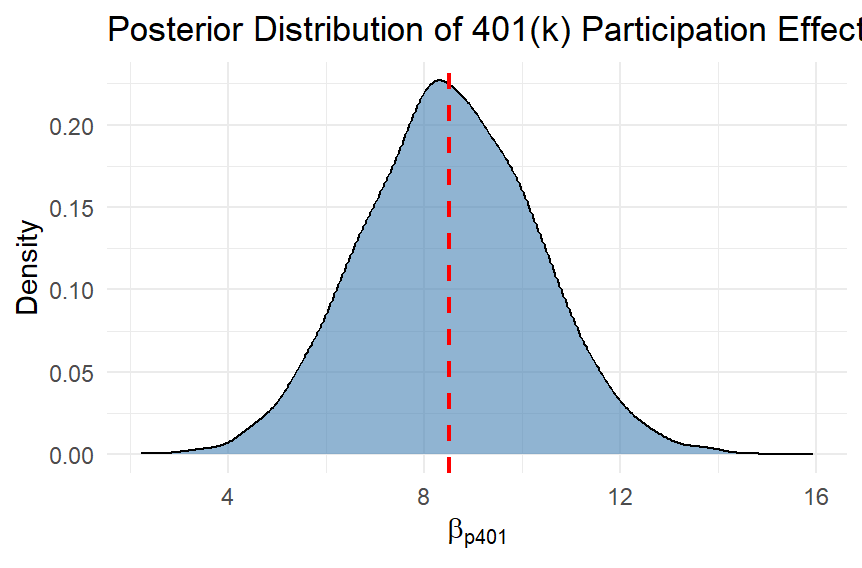
\includegraphics[width=340pt, height=200pt]{Chapters/chapter12/figures/FigP401k.png}
	\caption[List of figure caption goes here]{Posterior distribution: Local average treatment effect 401k participation on net financial assets using a Dirichlet process.}\label{fig12_2}
\end{figure}

	\item \textbf{Difference-in-Differences simulation continues}

Perform the simulation of the DiD example, and perform inference using the specification:

\[
Y_{it} = \alpha + \alpha_i + \phi_t + \tau_2 \,\big[ D_i \cdot \mathbbm{1}(t = 2) \big] + \epsilon_{it}.
\]

\textbf{Answer}

You can check that we get same results as in example in the main book.

\begin{tcolorbox}[enhanced,width=4.67in,center upper,
	fontupper=\large\bfseries,drop shadow southwest,sharp corners]
	\textit{R code. Difference-in-Differences: Simulation exercise}
	\begin{VF}
		\begin{lstlisting}[language=R]		
rm(list = ls()); set.seed(10101)
library(ggplot2); library(dplyr); library(fastDummies)
# Parameters
N_per_group <- 200          # units per group
T_periods    <- 2           # keep 2x2 for clarity
tau_true     <- 1         # ATT
sigma_eps    <- 0.5         # noise SD
# Panel index
id  <- rep(1:(2*N_per_group), each = T_periods)
t   <- rep(1:T_periods, times = 2*N_per_group)
# Group: treated (D=1) vs control (D=0)
D   <- rep(c(rep(0, N_per_group), rep(1, N_per_group)), each = T_periods)
# Post indicator (t=2 is post)
post <- as.integer(t == 2)
# Unit fixed effects (random heterogeneity)
alpha_i <- rnorm(2*N_per_group, 0, 0.8)
alpha   <- alpha_i[id]
# Time effects
phi_t <- c(0, -1.8)  # common decline from t=1 to t=2
phi   <- phi_t[t]
treat_effect <- tau_true * (D * post)
# Outcome
eps <- rnorm(length(id), 0, sigma_eps)
Y   <- alpha + phi + treat_effect + eps
did <- data.frame(id, t, D, post, Y)
plot_data <- did %>%
group_by(D, t) %>%
summarise(meanY = mean(Y), .groups = "drop") %>%
mutate(Group = ifelse(D == 1, "Treated", "Control"))
ggp <- ggplot(plot_data, aes(x = t, y = meanY, group = Group, linetype = Group)) +
geom_line(linewidth = 1) + geom_point() + scale_x_continuous(breaks = c(1, 2), labels = c("t = 1 (pre)", "t = 2 (post)")) + labs(x = "Time", y = "Mean outcome", title = "Synthetic DiD: Parallel Trends & No Anticipation") + theme_minimal(base_size = 12)
print(ggp)
# Bayesian inference: Model with interaction treatment x post period
post_fit1 <- MCMCpack::MCMCregress(Y ~ 1 + factor(id) + factor(t) + I(D * post), data = did, burnin = 100, mcmc = 1000)
tau_draws1 <- post_fit1[, "I(D * post)"]
quantile(tau_draws1, c(.025,.5,.975))
\end{lstlisting}
	\end{VF}
\end{tcolorbox}  

\item \textbf{Difference-in-Differences simulation continues II}

Note that another strategy to perform inference on the ATT is to estimate the saturated model
\[
Y_{it} = \sum_{t,d} \mu_{tl} \big[ D_{il} \cdot \mathbbm{1}(t = t) \big] + \epsilon_{it}, \quad t = 1, 2, \ d = 1, 0,
\]
and then use the posterior draws to compute
\[
\tau_2 = (\mu_{21} - \mu_{11}) - (\mu_{20} - \mu_{10}).
\]
Explain why inference on $\tau_2$ using this approach in the simulation setting shows that the posterior mean is similar to that from the previous approaches, but the level of uncertainty is higher.

\textbf{Answer}

There is more uncertainty because performing inference on $\tau_2$ uses four parameters in this setting, whereas in the previous we use only one parameter.

\begin{tcolorbox}[enhanced,width=4.67in,center upper,
	fontupper=\large\bfseries,drop shadow southwest,sharp corners]
	\textit{R code. Difference-in-Differences: Simulation exercise}
	\begin{VF}
		\begin{lstlisting}[language=R]
rm(list = ls()); set.seed(10101)
library(ggplot2); library(dplyr); library(fastDummies)
# Parameters
N_per_group <- 200          # units per group
T_periods    <- 2           # keep 2x2 for clarity
tau_true     <- 1           # ATT
sigma_eps    <- 0.5         # noise SD
# Panel index
id  <- rep(1:(2*N_per_group), each = T_periods)
t   <- rep(1:T_periods, times = 2*N_per_group)
# Group: treated (D=1) vs control (D=0)
D   <- rep(c(rep(0, N_per_group), rep(1, N_per_group)), each = T_periods)
# Post indicator (t=2 is post)
post <- as.integer(t == 2)
# Unit fixed effects (random heterogeneity)
alpha_i <- rnorm(2*N_per_group, 0, 0.8)
alpha   <- alpha_i[id]
# Time effects
phi_t <- c(0, -1.8)  # common decline from t=1 to t=2
phi   <- phi_t[t]
# No anticipation: effect is zero in pre, equals tau in post *only for treated*
treat_effect <- tau_true * (D * post)
# Outcome: Y_it(0) = alpha_i + phi_t + linear trend if you want; here just FE + shock
eps <- rnorm(length(id), 0, sigma_eps)
Y   <- alpha + phi + treat_effect + eps
did <- data.frame(id, t, D, post, Y)
# Calculating the means at each level, and then ATT
# ---- Build 2x2 cell indicators (no intercept model) ----
did$c_pre  <- as.integer(did$D == 0 & did$t == 1)
did$c_post <- as.integer(did$D == 0 & did$t == 2)
did$t_pre  <- as.integer(did$D == 1 & did$t == 1)
did$t_post <- as.integer(did$D == 1 & did$t == 2)
# Sanity check: each row must belong to exactly one cell
stopifnot(all(did$c_pre + did$c_post + did$t_pre + did$t_post == 1))
# ---- Bayesian saturated cell-mean model (compatible priors) ----
# No intercept: each coefficient IS a cell mean.
fit_cells <- MCMCpack::MCMCregress(
Y ~ 0 + c_pre + c_post + t_pre + t_post, data  = did, burnin = 1000, mcmc = 10000, thin = 5)
draws_cells <- as.matrix(fit_cells)
colnames(draws_cells)  # should be c("c_pre","c_post","t_pre","t_post", "sigma2")
# Posterior of the four cell means
mu_c_pre_draw  <- draws_cells[, "c_pre"]; mu_c_post_draw <- draws_cells[, "c_post"]
mu_t_pre_draw  <- draws_cells[, "t_pre"]; mu_t_post_draw <- draws_cells[, "t_post"]
# ATT = (mu_t,post - mu_t,pre) - (mu_c,post - mu_c,pre)
ATT_cells_draw <- (mu_t_post_draw - mu_t_pre_draw) - (mu_c_post_draw - mu_c_pre_draw)
quantile(ATT_cells_draw, c(.025, .5, .975))
\end{lstlisting}
	\end{VF}
\end{tcolorbox}  

\item Perform a simulation exercise to assess the ability of BETEL to identify the causal effect when an instrument is used to address the omission of relevant regressors. Illustrate the consequences of varying the dependence between the omitted regressor and the observed regressor.

\textbf{Answer}

We simulate the observed process $X_i = 0.5Z_i + e_i$, with the unobserved regressor defined as $W_i = H_i + \nu_i$, where 
\[
\begin{bmatrix}
	e_i \\
	\nu_i
\end{bmatrix}\sim N\left(\begin{bmatrix}
0\\
0
\end{bmatrix},\begin{bmatrix}
1 & \rho\\
\rho & 1
\end{bmatrix}\right).
\]
Thus, $\rho$ defines the degree of correlation between $X_i$ and $W_i$, and we perform two exercises with $\rho \in \{0.0, 0.7\}$. The variables $Z_i$ and $H_i$ are standard normal. The dependent variable is specified as 
\[
Y_i = 1 + 1.2X_i - 0.7W_i + \mu_i,
\]
where $\mu_i$ follows a mixture of two normal distributions with means $0.5$ and $-0.5$, and standard deviations $0.5$ and $1.2$. The sample size is 2{,}000, the burn-in is 1{,}000, and the number of MCMC draws retained after burn-in is 10{,}000. We adopt the default hyperparameter values provided in the \textit{betel} package. For comparison, we also perform the analysis under the assumption of no endogeneity using the package \textit{MCMCpack} using default values for the hyperparameters. 

The following code shows the implementation, and Figure~\ref{fig12_Omission} displays the posterior distributions. When $\rho = 0$, implying no association between the regressors, there are no endogeneity issues, and assuming exogeneity yields more efficient posterior estimates. In contrast, when $\rho = 0.7$, endogeneity arises, and assuming exogeneity produces a biased posterior distribution. BETEL performs relatively well in both settings, although it is less efficient.

\begin{tcolorbox}[enhanced,width=4.67in,center upper,
	fontupper=\large\bfseries,drop shadow southwest,sharp corners]
	\textit{R code. BETEL: Omission of a relevant regressor}
	\begin{VF}
		\begin{lstlisting}[language=R]
rm(list = ls()); set.seed(10101)
library(betel); library(ucminf)
# Simulate data
N <- 2000; d <- 2; k <- 2
gamma <- 0.5; beta <- c(1, 1.2, -0.7); rho <- 0.7
# Mixture
mum1 <- 1/2; mum2 <- -1/2
mu1 <- rnorm(N, mum1, 0.5); mu2 <- rnorm(N, mum2, 1.2)
mu <- sapply(1:N, function(i){sample(c(mu1[i], mu2[i]), 1, prob = c(0.5, 0.5))})
z <- rnorm(N) # Instrument
E <- MASS::mvrnorm(n = N, mu = c(0, 0), Sigma = matrix(c(1,rho,rho,1),2,2))
x <- gamma*z + E[,1] # Observed regressor
w <- rnorm(N) + E[,2] # Unobserved correlated regressor
X <- cbind(1, x, w)
y <- X%*%beta + mu
dat <- cbind(1, x, z) # Data
# Function g_i by row in BETEL
gfunc <- function(psi = psi, y = y, dat = dat) {
	X <- dat[,1:2]
	e <- y - X %*% psi
	E <- e %*% rep(1,d)
	Z <- dat[,c(1,3)]
	G <- E * Z;
	return(G)
}
nt <- round(N * 0.1, 0); # training sample size for prior
psi0 <- lm(y[1:nt]~x[1:nt])$coefficients # Starting value of psi = (theta, v), v is the slack parameter in CSS (2018)
names(psi0) <- c("alpha","beta")
psi0_ <- as.matrix(psi0) # Prior mean of psi 
Psi0_ <- 5*rep(1,k) # Prior dispersions of psi
lam0 <- .5*rnorm(d) # Starting value of lambda
nu <- 2.5 # df of the prior student-t
nuprop <- 15 # df of the student-t proposal
n0 <- 1000 # burn-in
m <- 10000 # iterations beyond burn-in
# MCMC ESTIMATION BY THE CSS (2018) method
psim2 <- betel::bayesetel(gfunc = gfunc, y = y[-(1:nt)], dat = dat[-(1:nt),], psi0 = psi0, lam0 = lam0, psi0_ = psi0_, Psi0_ = Psi0_, nu = nu, nuprop = nuprop,
controlpsi = list(maxiterpsi = 50, mingrpsi = 1.0e-8), #  list of parameters in maximizing likelihood over psi
controllam = list(maxiterlam = 50, # list of parameters in minimizing dual over lambda
mingrlam = 1.0e-7),
n0 = n0, m = m)
MCMCreg2 <- MCMCpack::MCMCregress(y~x)
\end{lstlisting}
	\end{VF}
\end{tcolorbox} 

\begin{figure}[h!]
	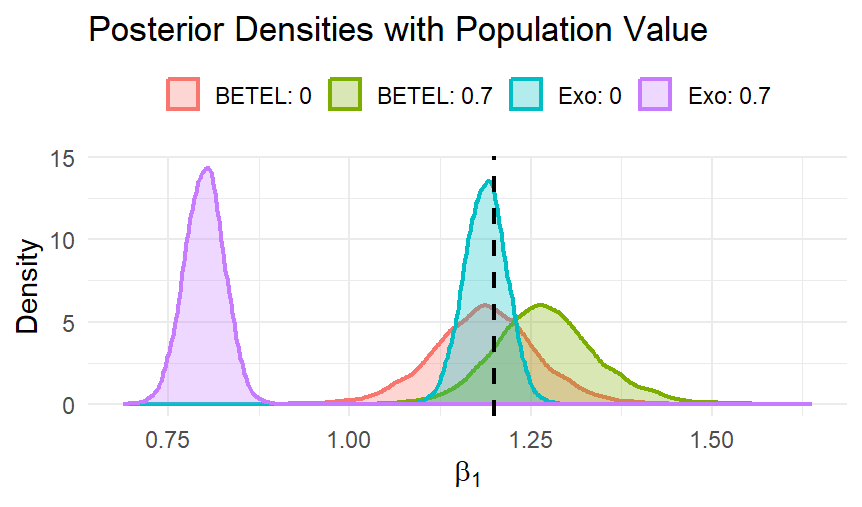
\includegraphics[width=340pt, height=200pt]{Chapters/chapter12/figures/FigOM.png}
	\caption[List of figure caption goes here]{Posterior distribution slope parameter given omission of relevant regressor: betel and MCMCregress}\label{fig12_Omission}
\end{figure}

	\item \textbf{Simultaneous causality continues}
	
	Use the demand–supply simulation and the moment conditions to infer the causal effect of a	10\% tax, implementing a BETEL algorithm from scratch. 

\textbf{Answer}

The following code shows how to program a BETEL from scratch for the demand-supply simulation exercise. Figure~\ref{fig12_Causal} displays the posterior distribution of the causal effect. The 95\% credible interval contains the population value, and the posterior mean lies close to it.

\begin{tcolorbox}[enhanced,width=4.67in,center upper,
	fontupper=\large\bfseries,drop shadow southwest,sharp corners]
	\textit{R code. BETEL: Simultaneous causality}
	\begin{VF}
		\begin{lstlisting}[language=R]
# Simulation
rm(list = ls()); set.seed(12345)
# Population parameters demand
B1 <- 5; B2 <- -0.5; B3 <- 0.8; B4 <- -0.4; B5 <- 0.7; SD <- 0.5
# Population parameters supply
A1 <- -2; A2 <- 0.5; A3 <- -0.4; SS <- 0.5
# Reduced form parameters
P0 <- (A1-B1)/(B2-A2); P2 <- -B3/(B2-A2); P3 <- -B4/(B2-A2); P1 <- A3/(B2-A2); P4 <- -B5/(B2-A2)
T0 <- B1+B2*P0; T2 <- B3+B2*P2; T3 <- B4+B2*P3; T1 <- B2*P1; T4 <- B5+B2*P4;
n <- 5000
ED <- rnorm(n, 0, SD); ES <- rnorm(n, 0, SS)
VP <- (ES-ED)/(B2-A2); UQ <- B2*VP+ED
y <- rnorm(n, 10, 1); pc <- rnorm(n, 5, 1); er <- rnorm(n, 15, 1); ps <- rnorm(n, 5, 1);
p <- P0+P1*er+P2*y+P3*pc+P4*ps+VP
q <- T0+T1*er+T2*y+T3*pc+T4*ps+UQ

### Supply ###
p_s  <- as.numeric(scale(p,  TRUE, TRUE))
er_s <- as.numeric(scale(er, TRUE, TRUE))

X <- cbind(1, p_s, er_s)  # k = 3  (STRUCTURAL: intercept, p, er)
Z <- cbind(1,
as.numeric(scale(y,  TRUE, TRUE)),
as.numeric(scale(pc, TRUE, TRUE)),
as.numeric(scale(ps, TRUE, TRUE)),
er_s)          # EXCLUDED instruments y,pc,ps, plus er

k <- ncol(X); d <- ncol(Z)

# Objective function
lambdafunc <- function(lambda, theta, q, X, Z){
	e <- as.numeric(q - X %*% theta); if (!all(is.finite(e))) return(1e300)
	G <- Z * e
	eta <- as.numeric(G %*% lambda); if (!all(is.finite(eta))) return(1e300)
	m <- max(eta); m + log(mean(exp(eta - m)))
}

# ----- Profile ETEL log-likelihood (use this in MH) -----
loglik_etel <- function(theta, q, X, Z){
	e <- as.numeric(q - X %*% theta); if (!all(is.finite(e))) return(-Inf)
	G <- Z * e
	op <- optim(par = rep(0, ncol(G)), fn = function(l){
		eta <- as.numeric(G %*% l); m <- max(eta)
		m + log(mean(exp(eta - m)))
	}, method="BFGS", control=list(maxit=2000))
	if (!is.finite(op$value)) return(-Inf)
	lam <- op$par
	eta <- as.numeric(G %*% lam)
	sum(eta) - length(e) * log(sum(exp(eta))) 
}
\end{lstlisting}
	\end{VF}
\end{tcolorbox} 

\begin{tcolorbox}[enhanced,width=4.67in,center upper,
	fontupper=\large\bfseries,drop shadow southwest,sharp corners]
	\textit{R code. BETEL: Simultaneous causality}
	\begin{VF}
		\begin{lstlisting}[language=R]
theta0 <- coef(lm(q ~ p_s + er_s))
# ----- MH using profile ETEL -----
b0 <- rep(0, k); B0 <- 1000*diag(k)
S <- 10000; burnin <- 2000; thin <- 5; tot <- S + burnin
BETA <- matrix(NA, tot, k); accept <- logical(tot)
step <- c(0.05, 0.02, 0.02)                  # preconditioned steps
BETA[1,] <- theta0
LL <- loglik_etel(BETA[1,], q, X, Z)
pb <- txtProgressBar(min=0, max=tot, style=3)
for(s in 2:tot){
	cand <- BETA[s-1,] + rnorm(k, 0, step)
	LLc  <- loglik_etel(cand, q, X, Z)
	priorRat <- mvtnorm::dmvnorm(cand, b0, B0, log=TRUE) -
	mvtnorm::dmvnorm(BETA[s-1,], b0, B0, log=TRUE)
	loga <- (LLc - LL) + priorRat
	if (is.finite(loga) && log(runif(1)) <= loga) {
		BETA[s,] <- cand; LL <- LLc; accept[s] <- TRUE
	} else {
		BETA[s,] <- BETA[s-1,]; accept[s] <- FALSE
	}
	if (s %% 200 == 0) {          # gentle adaptation
		acc <- mean(accept[(s-199):s])
		if (acc > 0.4) step <- step * 1.25
		if (acc < 0.15) step <- step / 1.25
	}
	setTxtProgressBar(pb, s)
}
close(pb)
cat("\nAcceptance rate:", mean(accept), "\n")
keep <- seq(burnin, tot, by = thin)
post_s <- BETA[keep, , drop=FALSE]   # posterior draws in scaled space
## ---------- Back-transform each draw to original scale ----------
p_mu <- mean(p);   p_sd <- sd(p); er_mu <- mean(er); er_sd <- sd(er)
alpha_draws <- cbind(
alpha0  = post_s[,1] - post_s[,2] * (p_mu/p_sd) - post_s[,3] * (er_mu/er_sd),
alphap  = post_s[,2] / p_sd,
alphaer = post_s[,3] / er_sd
)
## ---------- Summaries ----------
summ <- function(x) c(mean=mean(x), sd=sd(x), quantile(x, c(.025,.25,.5,.75,.975)))
cat("\nPosterior (original scale):\n")
print(rbind(
alpha0  = summ(alpha_draws[,"alpha0"]), alphap  = summ(alpha_draws[,"alphap"]), alphaer = summ(alpha_draws[,"alphaer"])))
cat("\nTrue (original scale):\n")
print(c(alpha0=A1, alphap=A2, alphaer=A3))
ElastSupPrice <- alpha_draws[,2]
#### Demand ####
y_s <- as.numeric(scale(y)); pc_s <- as.numeric(scale(pc))
ps_s <- as.numeric(scale(ps)); Xdem <- cbind(1, p_s, y_s, pc_s, ps_s) 
k <- ncol(Xdem); d <- ncol(Z); theta0 <- coef(lm(q ~ p_s + y_s + pc_s + ps_s))
\end{lstlisting}
	\end{VF}
\end{tcolorbox} 

\begin{tcolorbox}[enhanced,width=4.67in,center upper,
	fontupper=\large\bfseries,drop shadow southwest,sharp corners]
	\textit{R code. BETEL: Simultaneous causality}
	\begin{VF}
		\begin{lstlisting}[language=R]
# ----- MH using profile ETEL -----
b0 <- rep(0, k); B0 <- 1000*diag(k)
S <- 10000; burnin <- 2000; thin <- 5; tot <- S + burnin
BETAdem <- matrix(NA, tot, k); accept <- logical(tot)
step <- c(0.05, 0.02, 0.02); BETAdem[1,] <- theta0
LL <- loglik_etel(BETAdem[1,], q, X = Xdem, Z)
pb <- txtProgressBar(min=0, max=tot, style=3)
for(s in 2:tot){
	cand <- BETAdem[s-1,] + rnorm(k, 0, step)
	LLc  <- loglik_etel(cand, q, X = Xdem, Z)
	priorRat <- mvtnorm::dmvnorm(cand, b0, B0, log=TRUE) -
	mvtnorm::dmvnorm(BETAdem[s-1,], b0, B0, log=TRUE)
	loga <- (LLc - LL) + priorRat
	if (is.finite(loga) && log(runif(1)) <= loga) {
		BETAdem[s,] <- cand; LL <- LLc; accept[s] <- TRUE
	} else {
		BETAdem[s,] <- BETAdem[s-1,]; accept[s] <- FALSE
	}
	if (s %% 200 == 0) {   # gentle adaptation
		acc <- mean(accept[(s-199):s])
		if (acc > 0.4) step <- step * 1.25
		if (acc < 0.15) step <- step / 1.25
	}
	setTxtProgressBar(pb, s)
}
close(pb)
cat("\nAcceptance rate:", mean(accept), "\n")
keep <- seq(burnin, tot, by = thin)
postDem_s <- BETAdem[keep, , drop=FALSE] 
p_mu <- mean(p);   p_sd <- sd(p); y_mu <- mean(y); y_sd <- sd(y)
pc_mu <- mean(pc); pc_sd <- sd(pc); ps_mu <- mean(ps); ps_sd <- sd(ps)
alphaDem_draws <- cbind(
alpha0  = postDem_s[,1] - postDem_s[,2] * (p_mu/p_sd) - postDem_s[,3] * (y_mu/y_sd)
- postDem_s[,4] * (pc_mu/pc_sd) - postDem_s[,5] * (pc_mu/pc_sd),
alphap  = postDem_s[,2] / p_sd, alphay = postDem_s[,3] / y_sd, alphapc = postDem_s[,4] / pc_sd, alphaps = postDem_s[,5] / ps_sd)
summ <- function(x) c(mean=mean(x), sd=sd(x), quantile(x, c(.025,.25,.5,.75,.975)))
cat("\nPosterior (original scale):\n")
print(rbind(
alpha0  = summ(alphaDem_draws[,"alpha0"]), alphap  = summ(alphaDem_draws[,"alphap"]), alphay = summ(alphaDem_draws[,"alphay"]),
alphapc = summ(alphaDem_draws[,"alphapc"]), alphaps = summ(alphaDem_draws[,"alphaps"])))
cat("\nTrue (original scale):\n")
print(c(alpha0=B1, alphap=B2, alphay=B3, alphpc=B4, alphaps=B5))
ElastDemPrice <- alphaDem_draws[,2]; tax <- 0.1
CausalEffect <- (ElastSupPrice*ElastDemPrice)*log(1+tax)/(ElastSupPrice-ElastDemPrice) 
popCauEff <- (A2 * B2)/(A2 - B2) * log(1 + tax)
\end{lstlisting}
	\end{VF}
\end{tcolorbox} 

\begin{figure}[h!]
	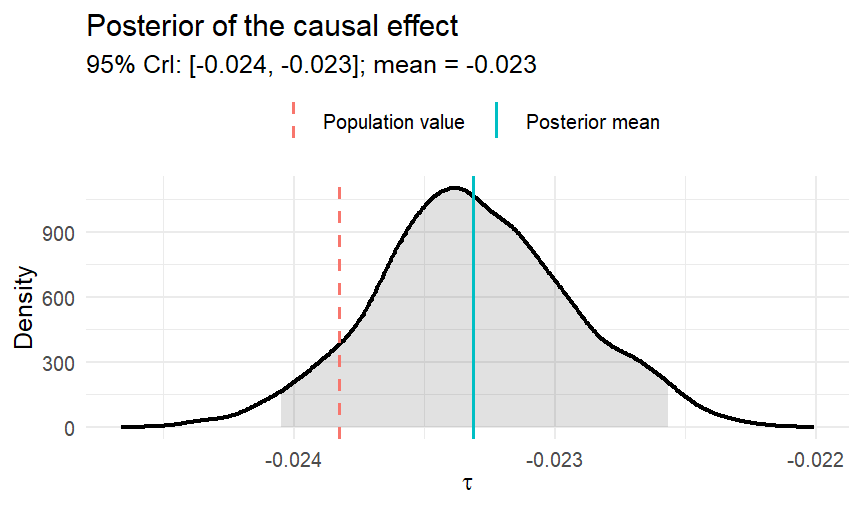
\includegraphics[width=340pt, height=200pt]{Chapters/chapter12/figures/fig12_SimCausality.png}
	\caption[List of figure caption goes here]{Posterior distribution causal effect: BETEL}\label{fig12_Causal}
\end{figure}

	\item Perform a simulation of the instrumental variable quantile regression, and then perform inference using the general Bayes posterior framework. Use the Laplace asymmetric distribution to simulate the stochastic error, such that 
\[
\int_{-\infty}^{0} f_{\tau}(\mu_i) \, d\mu_i = \tau,
\] 
which implies that the $\tau$-th quantile of $\mu_i$ is 0. In addition, let 
\[
q_{\tau}(Y_i \mid X_i, D_i) = \beta_0 + \beta_1 X_i + \beta_2 D_i
\] 
denote the $\tau$-th quantile regression function of $Y_i$ given $X_i$ and $D_i$, with $0 < \tau < 1$. Specifically, consider the model
\[
Y_i = \beta_{0\tau} + \beta_{1\tau} X_i + \beta_{2\tau} D_i + \mu_i,
\]
together with 
\[
D_i = \gamma Z_i + \delta \mu_i, \quad Z_i \sim N(0,1).
\]


\textbf{Answer:}

The following code shows how to perform inference in this simulation. The 95\% credible intervals encompass the population values, and the posterior means are also close to these values.

\begin{tcolorbox}[enhanced,width=4.67in,center upper,
	fontupper=\large\bfseries,drop shadow southwest,sharp corners]
	\textit{R code. Instrumental Variable Quantile Regression: General Bayes posteriors}
	\begin{VF}
		\begin{lstlisting}[language=R]
rm(list = ls()); set.seed(10101); library(quantreg)
### Simulation ####
# Asymmetric Laplace
rALD <- function(n, tau) {
	stopifnot(tau > 0, tau < 1)
	theta <- (1 - 2*tau) / (tau * (1 - tau))
	psi   <- 2 / (tau * (1 - tau))
	v  <- rexp(n, rate = 1)
	z  <- rnorm(n)
	mu <- theta * v + sqrt(psi * v) * z
	return(mu)
}
## --- Simulator for a given tau ---
simulate_qr <- function(n = 5000, tau = 0.5,
beta0 = 0.7,
beta1_tau = 1.5,
beta2_tau = 1,
gamma = 1,
delta = 0.5) {
	# Nonnegative regressor stabilizes intercept & preserves tau-ordering of slopes
	x <- runif(n, 0, 1)
	# optional: anchor a portion at 0 to pin intercept
	x[sample.int(n, size = round(0.1*n))] <- 0
	mu <- rALD(n, tau = tau) # ALD error
	z <- rnorm(n) # Instrument
	d <- gamma * z + delta * mu
	y <- beta0 + beta1_tau * x + beta2_tau * d + mu
	df <- data.frame(y, x, d, z)
}
tau <- 0.75
df <- simulate_qr(tau = tau, beta0 = 1, beta1_tau = 1,
beta2_tau = 1, gamma = 1, delta = 1, n = 5000)
Reg <- MCMCpack::MCMCquantreg(y~x+d, data = df, tau = tau)
summary(Reg)
summary(rq(y ~ x + d, tau = tau, data = df))
LossFunct <- function(par, tau, y, z, x, d){
	n <- length(y)
	X <- cbind(1, x, d)
	Z <- cbind(1, x, z)
	Ind <- as.numeric(y <= X%*%par) 
	gn <- colMeans((tau - Ind) * Z)
	Wni <- lapply(1:n, function(i) {Z[i,] %*% t(Z[i,])}) 
	Wn <- 1 / (tau * (1 - tau)) * solve(Reduce("+", Wni)/n)
	Ln <- - 0.5 * n * t(gn) %*% Wn %*% gn
	return(Ln)
}
par0 <- rnorm(3)
LossFunct(par = par0, tau = tau, y = df$y, z = df$z, x = df$x, d = df$d)
\end{lstlisting}
	\end{VF}
\end{tcolorbox} 

\begin{tcolorbox}[enhanced,width=4.67in,center upper,
	fontupper=\large\bfseries,drop shadow southwest,sharp corners]
	\textit{R code. Instrumental Variable Quantile Regression: General Bayes posteriors}
	\begin{VF}
		\begin{lstlisting}[language=R]
# ----- MH using Ln -----
k <- 3
b0 <- rep(0, k); B0 <- 1000*diag(k)
S <- 5000; burnin <- 6000; thin <- 5; tot <- S + burnin
BETA <- matrix(NA, tot, k); accept <- logical(tot)
step <- 0.05
BETA[1,] <- par0
LL <- LossFunct(par = BETA[1,], tau = tau, y = df$y, z = df$z, x = df$x, d = df$d)
pb <- txtProgressBar(min=0, max=tot, style=3)
for(s in 2:tot){
	cand <- BETA[s-1,] + rnorm(k, 0, step)
	LLc  <- LossFunct(par = cand, tau = tau, y = df$y, z = df$z, x = df$x, d = df$d)
	priorRat <- mvtnorm::dmvnorm(cand, b0, B0, log=TRUE) -
	mvtnorm::dmvnorm(BETA[s-1,], b0, B0, log=TRUE)
	loga <- (LLc - LL) + priorRat
	if (is.finite(loga) && log(runif(1)) <= loga) {
		BETA[s,] <- cand; LL <- LLc; accept[s] <- TRUE
	} else {
		BETA[s,] <- BETA[s-1,]; accept[s] <- FALSE
	}
	if (s <= burnin && s %% 200 == 0) {          
		acc <- mean(accept[(s-199):s])
		if (acc > 0.4) step <- step * 1.25
		if (acc < 0.15) step <- step / 1.25
	}
	setTxtProgressBar(pb, s)
}
close(pb)
cat("\nAcceptance rate:", mean(accept), "\n")
keep <- seq(burnin, tot, by = thin)
post <- BETA[keep, , drop=FALSE]   # posterior draws in scaled space
colnames(post) <- c("beta0","beta_x","beta_d")
# Posterior summaries
post_mean <- colMeans(post)
post_ci   <- apply(post, 2, quantile, c(0.025, 0.975))
round(post_mean, 3); round(post_ci, 3)
\end{lstlisting}
	\end{VF}
\end{tcolorbox} 

\item \textbf{Example: Doubly robust Bayesian inference continues}

Perform a simulation exercise to assess the consequences of misspecifying the propensity score function and the outcome regression in doubly robust Bayesian inference.

\textbf{Answer:}

Let us simulate the process 
\[
\eta^{\pi}_i = -0.3 + 0.8X_{i1} - 0.5X_{i2} + 0.7X_{i3} + 0.7X_{i1}X_{i3} + 0.5sin(X_{i1}), 
\]
\[
\eta^{m}_i = -0.2 + 0.6D_i + 0.5X_{i1} - 0.4X_{i2} + 0.3X_{i3} + 0.6X_{i1}^2 - 0.5X_{i1}X_{i2},
\]
where $X_{1}\sim N(0,1)$, $X_{2}\sim \mathrm{Bernoulli}(0.5)$, and $X_{3}\sim U(-1,1)$, and the sample size is 2,000.

The following code implements the algorithm.

\begin{tcolorbox}[enhanced,width=4.67in,center upper,
	fontupper=\large\bfseries,drop shadow southwest,sharp corners]
	\textit{R code. Doubly robust Bayesian inference: Misspecified simulation}
	\begin{VF}
		\begin{lstlisting}[language=R]
rm(list = ls()); set.seed(123); library(glmnet)

## simulate covariates
n  <- 2000
X1 <- rnorm(n)                 # continuous
X2 <- rbinom(n, 1, 0.5)        # binary
X3 <- runif(n, -1, 1)          # continuous
Z <- cbind(X1, X2, X3)
# True propensity and outcome
logit <- function(t) 1/(1+exp(-t))
true_pi  <- function(X){ logit(-0.3 + 0.8*X[,1] -0.5*X[,2] + 0.7*X[,3] + 0.7*X[,1]*X[,3] + 0.5*sin(X[,1])) }
true_eta <- function(d,X){ -0.2 + 0.6*d + 0.5*X[,1] -0.4*X[,2] + 0.3*X[,3] + 0.6*(X[,1]^2) - 0.5*X[,1]*X[,2] }
true_p   <- function(d,X){ logit(true_eta(d,X)) }
ATE  <- mean(true_p(1,Z) - true_p(0,Z))
pi <- true_pi(Z)
D  <- rbinom(n,1,pi)
P  <- true_p(D,Z)
Y  <- rbinom(n,1,P)
dat <- data.frame(Y, D, X1, X2 = factor(X2), X3)
######### Doubly Robust Bayesian: Implementation #########
# OK specification propensity score
Z <- cbind(X1, X2, X3, X1*X3, sin(X1)); p <- dim(Z)[2]
covars <- c("X1","X2","X3", "X1X3", "sinX1")
# # OK specification outcome regression
# Z <- cbind(X1, X2, X3, X1*X2, X1^2); p <- dim(Z)[2]
# covars <- c("X1","X2","X3", "X1X2", "X12")
cvfit <- cv.glmnet(Z, D, family = "binomial", alpha=1, nfolds = 10) # lasso,min
ps.coef <- coef(cvfit, s = "lambda.min")[0:p+1]
ps_hat <- predict(cvfit, newx = Z, s = "lambda.min",type = "response")
ps_hat <- pmin(pmax(ps_hat, 1e-6), 1 - 1e-6)
# Riesz representer
riesz_fun <- function(d, ps) d/ps - (1 - d)/(1 - ps)
# GP model
make_gp <- function(X_train, y_bin, use_correction = FALSE, gamma_scaled = NULL,
approx_method = gplite::approx_laplace(),
init_lscale = 0.3) {
	stopifnot(length(y_bin) == nrow(X_train))
	cf_se <- gplite::cf_sexp(vars = colnames(X_train), lscale = init_lscale, magn = 1, normalize = TRUE)
	cfs <- list(cf_se)
	if (use_correction) {
		stopifnot(!is.null(gamma_scaled))
		cf_lin <- gplite::cf_lin(vars = "gamma", magn = 1, normalize = FALSE)
		cfs <- list(cf_se, cf_lin)
	}
	gp <- gplite::gp_init(cfs = cfs, lik = gplite::lik_bernoulli(), approx = approx_method)
	gp <- gplite::gp_optim(gp, x = X_train, y = y_bin, maxiter = 1000, restarts = 3, tol = 1e-05)
	return(gp)
}
\end{lstlisting}
\end{VF}
\end{tcolorbox} 

\begin{tcolorbox}[enhanced,width=4.67in,center upper,
fontupper=\large\bfseries,drop shadow southwest,sharp corners]
\textit{R code. Doubly robust Bayesian inference: Simulation exercise}
\begin{VF}
\begin{lstlisting}[language=R]	
posterior_draws_prob <- function(gp, X_test, ndraws = 5000) {
	out <- gplite::gp_draw(gp, xnew = X_test, draws = ndraws, transform = TRUE, target = FALSE, jitter = 1e-6)
	return(t(out))
}
# Main function
run_trim <- function(t_trim = 0.10, N_post = 5000, h_r = 1/2, cor_size = 1) {
	# Trim by estimated PS
	keep <- which(ps_hat >= t_trim & ps_hat <= (1 - t_trim))
	n_eff <- length(keep)
	if (n_eff < 50) stop("Too few observations after trimming.")
	Yk  <- Y[keep]
	Dk  <- D[keep]
	Zk  <- Z[keep, , drop = FALSE]
	psk <- ps_hat[keep]
	# Riesz representer and sigma_n choice
	gamma_k <- riesz_fun(Dk, psk)
	sigma_n <- cor_size * (log(n_eff) / ( (n_eff)^(h_r) * mean(abs(gamma_k)) ))
	gamma_scaled <- sigma_n * gamma_k
	# Training inputs for GP: [Z, D] and, if corrected, an extra column 'gamma'
	X_train_nc <- data.frame(Zk)
	X_train_nc$D <- Dk
	colnames(X_train_nc) <- c(covars, "D")
	X_train_c <- X_train_nc
	X_train_c$gamma <- gamma_scaled
	# Test inputs: for each i, (Z_i, d=0) and (Z_i, d=1)
	X_t0 <- X_train_nc; X_t0$D <- 0
	X_t1 <- X_train_nc; X_t1$D <- 1
	X_t0c <- X_t0; X_t1c <- X_t1
	X_t0c$gamma <- sigma_n * riesz_fun(0, psk)   
	X_t1c$gamma <- sigma_n * riesz_fun(1, psk) 
	# GP WITHOUT prior correction #
	gp_nc <- make_gp(X_train = X_train_nc, y_bin = Yk, use_correction = FALSE)
	# joint draws for [m(Z,0); m(Z,1)]
	M_nc_0 <- posterior_draws_prob(gp_nc, X_t0, ndraws = N_post)  # N_post x n_eff
	M_nc_1 <- posterior_draws_prob(gp_nc, X_t1, ndraws = N_post)
	# observed arm probabilities
	M_nc_obs <- ifelse(matrix(Dk, nrow = N_post, ncol = n_eff, byrow = TRUE) == 1, M_nc_1, M_nc_0)
	# GP WITH prior correction #
	gp_c <- make_gp(X_train = X_train_c, y_bin = Yk, use_correction = TRUE, gamma_scaled = gamma_scaled)
	M_c_0 <- posterior_draws_prob(gp_c, X_t0c, ndraws = N_post)
	M_c_1 <- posterior_draws_prob(gp_c, X_t1c, ndraws = N_post)
	M_c_obs <- ifelse(matrix(Dk, nrow = N_post, ncol = n_eff, byrow = TRUE) == 1, M_c_1, M_c_0)
\end{lstlisting}
\end{VF}
\end{tcolorbox} 

\begin{tcolorbox}[enhanced,width=4.67in,center upper,
fontupper=\large\bfseries,drop shadow southwest,sharp corners]
\textit{R code. Doubly robust Bayesian inference: Simulation exercise}
\begin{VF}
\begin{lstlisting}[language=R]	
	# Bayesian bootstrap weights #
	W <- matrix(rexp(N_post * n_eff, rate = 1), nrow = N_post)
	W <- W / rowSums(W)
	# ATEs
	# (1) Unadjusted Bayes
	Ate_nc_draws <- rowSums((M_nc_1 - M_nc_0) * W)
	# (2) Prior-adjusted Bayes
	Ate_c_draws  <- rowSums((M_c_1 - M_c_0) * W)
	# (3) DR Bayes (posterior recentering)
	# Pre-centering using UNcorrected GP posterior means
	mu_nc_diff <- colMeans(M_nc_1 - M_nc_0)                
	mu_nc_obs  <- colMeans(M_nc_obs)                       
	ATE_dr_pre <- mean(mu_nc_diff + gamma_k * (Yk - mu_nc_obs))
	# Recenter draws using corrected GP draws
	DR_rec_1 <- (matrix(gamma_k, nrow = N_post, ncol = n_eff, byrow = TRUE)) * (matrix(Yk, nrow = N_post, ncol = n_eff, byrow = TRUE) - M_c_obs)
	# The first component is \tau_{\eta}^s in Algorithm 1
	# The second component is \hat{m} a scalar. This has positive sign because
	# minus x minus, the bias is with minus, and then, this component enters with minus in the bias term
	# The third component is \gamma_k x (y-m(d,x)), m(d,x) is with prior correction
	# The fourth component is m(1,x)-m(0,x) also with correction in the prior
	Ate_drb_draws <- rowSums((M_c_1 - M_c_0) * W) + ATE_dr_pre - rowSums(DR_rec_1) / n_eff - rowSums(M_c_1 - M_c_0) / n_eff
	
	qfun <- function(x) {
		qs <- quantile(x, c(0.025, 0.975))
		c(mean   = mean(x), 	median = median(x), lo = qs[1],	hi = qs[2],	len = diff(qs)
		)
	}	
	vals <- list(
	Bayes      = qfun(Ate_nc_draws),
	`PA Bayes` = qfun(Ate_c_draws),
	`DR Bayes` = qfun(Ate_drb_draws)
	)
	out_df <- as.data.frame(do.call(rbind, vals), check.names = FALSE)
	list(t_trim = t_trim, results = out_df)
}
N_post <- 5000
h_r    <- 1/2
cor_size <- 1
trim <- 0.05
res_list <- run_trim(t_trim = trim, N_post = N_post, h_r = h_r, cor_size = cor_size)
print(res_list$results)
\end{lstlisting}
\end{VF}
\end{tcolorbox} 


\end{enumerate}